

%%
%% This is file `sample-manuscript.tex',
%% generated with the docstrip utility.
%%
%% The original source files were:
%%
%% samples.dtx  (with options: `manuscript')
%% 
%% IMPORTANT NOTICE:
%% 
%% For the copyright see the source file.
%% 
%% Any modified versions of this file must be renamed
%% with new filenames distinct from sample-manuscript.tex.
%% 
%% For distribution of the original source see the terms
%% for copying and modification in the file samples.dtx.
%% 
%% This generated file may be distributed as long as the
%% original source files, as listed above, are part of the
%% same distribution. (The sources need not necessarily be
%% in the same archive or directory.)
%%
%% The first command in your LaTeX source must be the \documentclass command.

\documentclass[manuscript,screen,review]{acmart}

\graphicspath{{./}}

\usepackage[main = greek, english]{babel} % For Greek language
\newcommand{\img}[1]
{
    \begin{center}
        \fcolorbox{black}{white}{\includegraphics[height=20em]{#1}}
    \end{center}

}
\usepackage{hyperref}
\usepackage{listings}
\usepackage{graphicx}
\usepackage{float}

% Helper Macros

\newcommand{\en}[1]{\foreignlanguage{english}{#1}}
\newcommand{\src}[1]{{\tt\en{#1}}}

%%
%% End of file `acmart.

\newcommand{\question}[1] % This is what you will use to create a new question
{
\par\noindent % Creates a new unindented paragraph
\phantomsection % Needed for hyperref compatibility with the \addcontensline command
\todo[inline, color=YellowOrange]{\textbf{#1}} % Uses the todonotes package to create a fancy box to put the question
\vspace{1em} % White space after the question before the start of the answer
}


%%
%% \BibTeX command to typeset BibTeX logo in the docs
\AtBeginDocument{%
  \providecommand\BibTeX{{%
    \normalfont B\kern-0.5em{\scshape i\kern-0.25em b}\kern-0.8em\TeX}}}

%% Rights management information.  This information is sent to you
%% when you complete the rights form.  These commands have SAMPLE
%% values in them; it is your responsibility as an author to replace
%% the commands and values with those provided to you when you
%% complete the rights form.
% \setcopyright{}
% \copyrightyear{2023}
% \acmYear{}
% \acmDOI{}

%%
%% Submission ID.
%% Use this when submitting an article to a sponsored event. You'll
%% receive a unique submission ID from the organizers
%% of the event, and this ID should be used as the parameter to this command.
%%\acmSubmissionID{123-A56-BU3}

%%
%% The majority of ACM publications use numbered citations and
%% references.  The command \citestyle{authoryear} switches to the
%% "author year" style.
%%
%% If you are preparing content for an event
%% sponsored by ACM SIGGRAPH, you must use the "author year" style of
%% citations and references.
%% Uncommenting
%% the next command will enable that style.
%%\citestyle{acmauthoryear}

%%
%% end of the preamble, start of the body of the document source.
\begin{document}

%%
%% The "title" command has an optional parameter,
%% allowing the author to define a "short title" to be used in page headers.
\title{Εφαρμογή Διαχείρισης Σταθμών Επαναφόρτισης Ηλεκτρικών Αυτοκινήτων  \\ Εργασία στα πλαίσια του μαθήματος Βάσεις Δεδομένων (2023-24)}

%%
%% The "author" command and its associated commands are used to define
%% the authors and their affiliations.
%% Of note is the shared affiliation of the first two authors, and the
%% "authornote" and "authornotemark" commands
%% used to denote shared contribution to the research.



%%
%% By default, the full list of authors will be used in the page
%% headers. Often, this list is too long, and will overlap
%% other information printed in the page headers. This command allows
%% the author to define a more concise list
%% of authors' names for this purpose.

\author{Θεοχάρης Λάμψας, \en{up1083994}}

% \email{}
\affiliation{%
  \institution{Tμήμα Ηλεκτρολόγων Μηχανικών και Τεχνολογίας Υπολογιστών, Πανεπιστήμιο Πατρών}
 % \streetaddress{}
  %\city{ }
 % \state{}
  %\country{}
  %\postcode{}
}


%%
%% The abstract is a short summary of the work to be presented in the
%% article.
\begin{abstract}
\newline
 \en{Command Line Interface } εφαρμογή 
 Η συγκεκριμένη βάση δεδομένων μοντελοποιεί μια εφαρμογή
διαχείρισης σταθμών επαναφόρτισης ηλεκτρικών αυτοκινήτων
 \end{abstract}

%%
%% The code below is generated by the tool at http://dl.acm.org/ccs.cfm.
%% Please copy and paste the code instead of the example below.
%%


%%
%% Keywords. The author(s) should pick words that accurately describe
%% the work being presented. Separate the keywords with commas.
% \keywords{βάσεις δεδομένων, σχεδιασμός μιας βάσης, διάγραμμα οντοτήτων-συσχετίσεων, σχεσιακό σχήμα, επικοινωνία με την βάση, \en{SQL}}

%%
%% This command processes the author and affiliation and title
%% information and builds the first part of the formatted document.
\maketitle

\newpage

\section{Περίληψη}

 
 Η συγκεκριμένη βάση δεδομένων μοντελοποιεί μια εφαρμογή διαχείρισης σταθμών επαναφόρτισης 
 ηλεκτρικών αυτοκινήτων. Πιο συγκεκριμένα, παρέχει πολλές υπηρεσίες στον χρήστη της εφαρμογής, 
 ο οποίος αφού δημιουργήσει έναν λογαριασμό, έχει την δυνατότητα να εισάγει στην βάση 
 ηλεκτρικά αυτοκίνητα, να κλείσει ραντεβού με κάποιον σταθμό για την φόρτιση του αυτοκινήτου 
 του, να ψάξει για συνεργαζόμενους σταθμούς σε όποια περιοχή θέλει, αλλά και να εισάγει στην 
 εφαρμογή τραπεζικές κάρτες, ώστε να διευκολύνει τις πληρωμές του.
 
 Ο χρήστης στην συνέχεια μπορεί να επεξεργαστεί όλα τα εισηγμένα στην βάση δεδομένα
 του. Είναι ικανός λοιπόν να επεξεργαστεί αλλά και να διαγράψει τα αυτοκίνητα του, 
 τα ραντεβού του, αλλά και τις τραπεζικές κάρτες του.
 
\section{Μεθοδολογία}

 
 Για την δημιουργία της βάσης δεδομένων πρώτο βήμα αποτέλεσε η κατασκευή του μικρόκοσμου, 
 ο οποίος περιγράφει τις λειτουργίες που η βάση καλείται να υλοποιεί, καθιστώντας τον 
 καθοριστικό παράγοντα για οποιαδήποτε εξέλιξη της υλοποίησης.
 
 Έτσι λοιπόν, ο μικρόκοσμος αποτελείται από τις παρακάτω οντότητες, με την κάθε μια από
 αυτές να περιγράφεται από τα γνωρίσματά της:
 
 \begin{enumerate}
	\item ιδιοκτήτης του ηλεκτρικού αυτοκινήτου
	\begin{itemize}
		\item όνομα
		\item επίθετο
		\item \en{id}
		\item \en{email}
		\item τηλέφωνο
		\item τόπος
		\item ημερομηνία δημιουργίας λογαριασμού
	\end{itemize}
	\item ηλεκτρικό αυτοκίνητο
	\begin{itemize}
		\item πινακίδες
		\item μάρκα
		\item μοντέλο
		\item έτος κατασκευής αυτοκινήτου
	\end{itemize}
	\item σταθμός επαναφόρτισης
	\begin{itemize}
		\item \en{id} σταθμού
		\item τόπος
		\item διεύθυνση
		\item τηλέφωνο επικοινωνίας
		\item θέσεις φόρτισης
	\end{itemize}
	\item θέση φόρτισης 
	\begin{itemize}
		\item αριθμός θέσης
		\item κατειλημμένη ή ελεύθερη
		\item τύπος φορτιστή
		\item χρέωση ανά τύπο φορτιστή
	\end{itemize}
 \newpage
	\item φόρτιση
	\begin{itemize}
		\item αριθμός φόρτισης
		\item ενέργεια φόρτισης (σε \en{kWh})
		\item συνολικό κόστος φόρτισης
		\item ημερομηνία φόρτισης
		\item ώρα έναρξης φόριτσης
		\item ώρα λήξης φόρτισης
	\end{itemize}
	\item ραντεβού για φόρτιση
	\begin{itemize}
		\item αριθμός ραντεβού
		\item ώρα έναρξης
	\end{itemize}
	\item πληρωμή φόρτισης
	\begin{itemize}
		\item ποσό πληρωμής
		\item τρόπος πληρωμής
	\end{itemize}
	\item κριτική σε σταθμό
	\begin{itemize}
		\item \en{id} κριτικής
		\item αριθμός αστεριών κριτικής (1 έως 5)
		\item ημερομηνία κριτικής
	\end{itemize}
	\item τραπεζική κάρτα πληρωμών
	\begin {itemize}
		\item ονοματεπώνυμο κατόχου 
		\item αριθμός κάρτας
		\item ημερομηνία λήξης
		\item \en{cvc}
	\end{itemize}
 \end{enumerate}
	
Ταυτόχρονα, οι σχέσεις μεταξύ των οντοτήτων διαμορφώνονται ως εξής:
		
\begin{enumerate}
	\item ο ιδιοκτήτης κατέχει αυτοκίνητα
	\item ο ιδιοκτήτης πηγαίνει σε έναν σταθμό με κάποιο από τα αυτοκίνητα του
	\item ο κάθε σταθμός περιλαμβάνει θέσεις φόρτισης
	\item ο ιδιοκτήτης μπορεί να κλέισει ραντεβού για φόρτιση σε συγκεκριμένη ώρα και μέρα
	\item το αυτοκίνητο φορτίζεται
	\item μετά το πέρας της φόρτισης ο ιδιοκτήτης εκτελεί μια πληρωμή
	\item ο ιδιοκτήτης αποθηκεύει την κάρτα του στην εφαρμογή για προπληρωμή
	\item ο ιδιοκτήτης ασκεί κριτική στον σταθμό
\end{enumerate}

Κάποια παραπάνω σχόλια αναφορικά με τον μικρόκοσμο:
Κάθε ραντεβού είναι άρρηκτα συνδεδεμένο με μια φόρτιση, η οποία με την σειρά της είναι άρρηκτα
συνδεδεμένη με μια πληρωμή, καθώς κάθε ραντεβού, όταν φτάσει η αποθηκευμένη μέρα και ώρα 
«μετατρέπεται» σε φόρτιση, ενώ μετά από κάθε φόρτιση ακολουθεί η πληρωμή. Επιπλέον, σε περίπτωση 
που συμβεί φόρτιση έχοντας προηγηθεί ραντεβού, μια θέση φόρτισης κατοχυρώνεται για την μέρα και
ώρα του ραντεβού, διαφορετικά η θέση φόρτισης κατοχυρώνεται την στιγμή της φόρτισης.

\newpage
Παρακάτω φαίνεται το διάγραμμα \en{erd}, το οποίο αναπαριστά τον μικρόκοσμο πλήρως:

\begin{figure}[H]
    \centering
    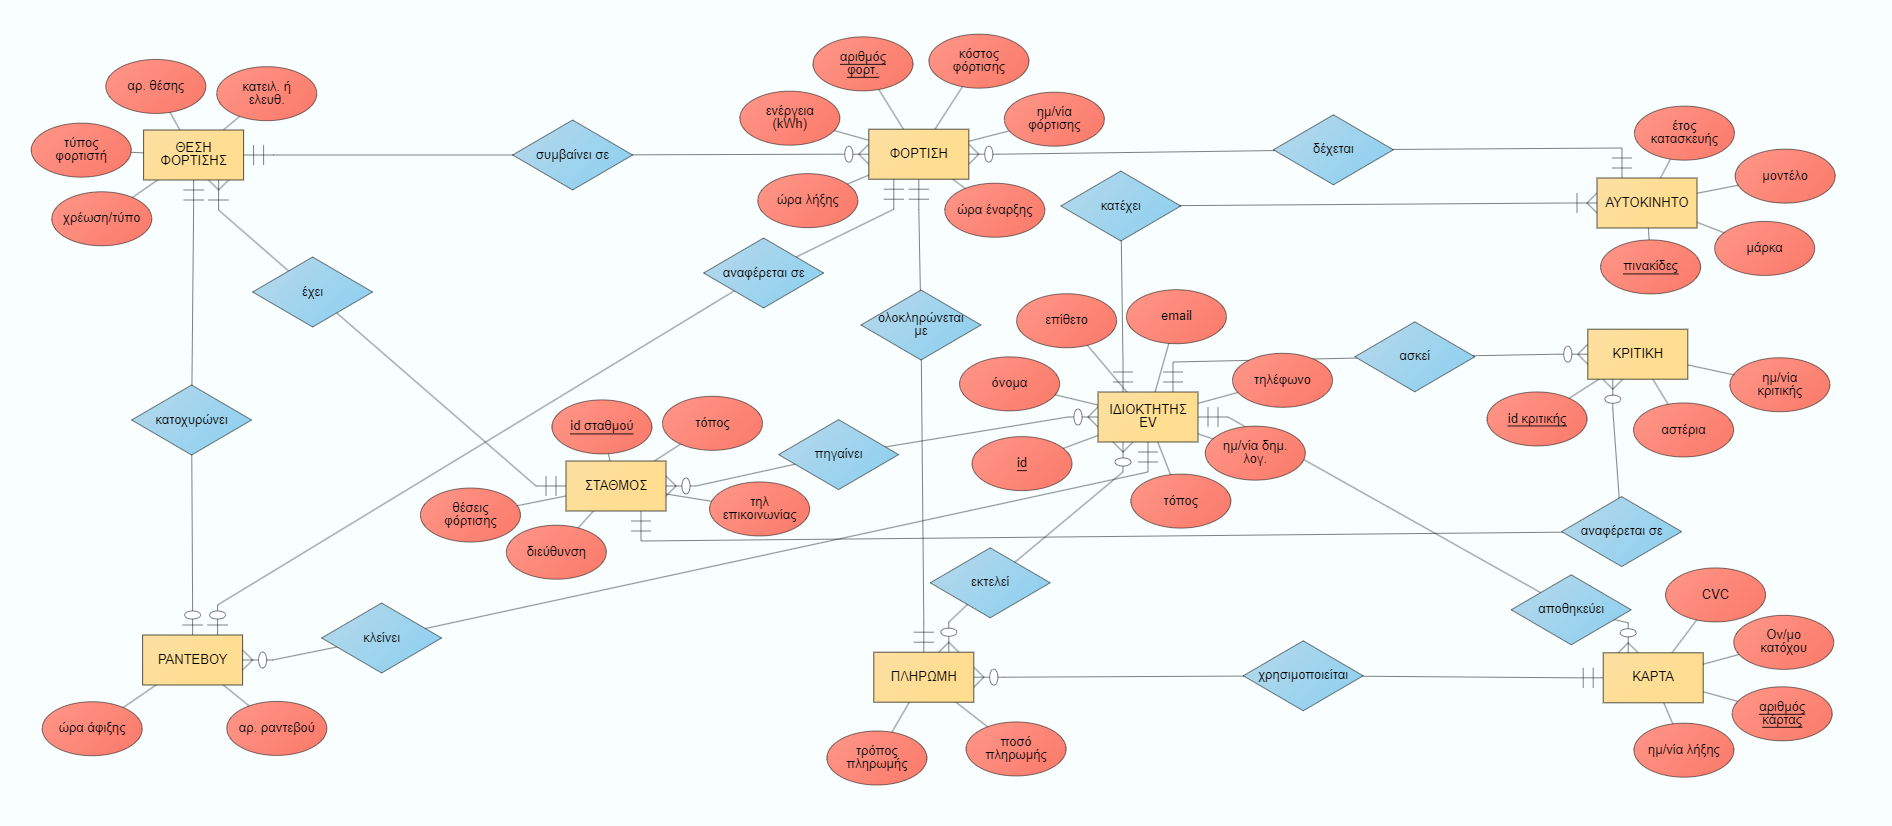
\includegraphics[width=1.1\textwidth]{./Διάγραμμα οντοτήτων συσχετίσεων (τελικό)_3.png}
    \caption{Διάγραμμα οντοτήτων - συσχετίσεων}
\end{figure}
\newpage
Μετά την δημιουργία του μικροκόσμου αλλά και την αναπαράστασή του μέσω του διαγράμματος
οντοτήτων-συσχετίσεων, σειρά έχει η dημιουργία του σχεσιακού μοντέλου:

\begin{figure}[H]
    \centering
    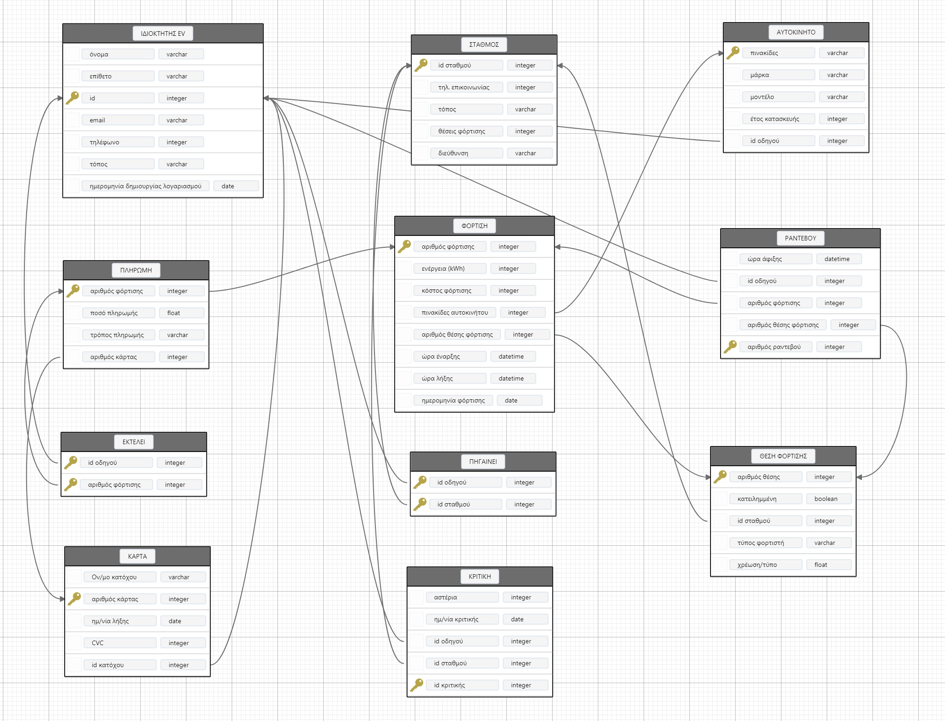
\includegraphics[width=1.1\textwidth]{./schema_final.png}
    \caption{Σχεσιακό Μοντέλο}
\end{figure}

\newpage

\section {Αξιολόγηση}


Το συγκεριμένο πρόγραμμα δεν υλοποιεί τόσο καλά τα ραντεβού των ιδιοκτητών για φόρτιση των οχημάτων 
τους καθώς δεν έχει υλοποιηθεί κάποια συνάρτηση για μετατροπή ενός μελλοντικού ραντεβού σε παροντική 
φόρτιση, με αποτέλεσμα το πρόγραμμα να μην γνωρίζει ποια θέση φόρτισης είναι κατειλημμένη ανά πάσα στιγμή.

\section {Δεδομένα}


Για την περάτωση της εργασίας αυτής χρειάστηκε αρκετές φορές να συλλέξω δεδομένα, κυρίως για την 
εισαγωγή στην βάση δεδομένων τυχαίων στοιχείων με την μορφή εγγραφών, με σκοπό την ύπαρξη λειτουργικότητας
είτε στις ερωτησεις (\en{queries}), είτε στην γενική χρήση της εφαρμογής από τον χρήστη. Ο τρόπος που
αντιμετώπιζα αυτό το πρόβλημα είναι με την εισαγωγή δεδομένων σε αρχεία τύπου \en{.txt} και στην συνέχεια
με χρήση της γλώσσας προγραμματισμού \en{python}, με την οποία εισήγαγα τα δεδομένα αυτά στην βάση.
Για παράδειγμα, για εισαγωγή 100 τυχαίων ονομάτων στην βάση άντλησα δεδομένα από τον ιστότοπο: 
\en{https://1000randomnames.com/}, για εισαγωγή 100 τυχαίων ηλεκτρικών αυτοκίνητων από το:
\en{https://ev-database.org/cheatsheet/range-electric-car}, ενώ για την εισαγωγή 20 σταθμών 
επαναφόρτισης ηλεκτρικών αυτοκινήτων από το: 
\en{https://www.autonomous.gr/stathmoi-fortisis-ilektrikon-ochimaton-stin-ellada/}.


\section{Προγραμμα}


Για την ανάπτυξη της εφαρμογής, έγινε χρήση της γλώσσας \en{python}, αλλά και της γλώσσας \en{sqlite} μέσω
της \en{python}, κάνοντας χρήση της εντολής \en{import sqlite3 as sql}.

Όλος ο κώδικας είναι χωρσιμένος σε 4 μέρη:

\begin{enumerate}
	\item \en{db\_init.py} : Αρχικοποίηση της βάσης \en{ev.db}
	\item \en{db\_fill.py} : Γέμισμα της βάσης με τυχαία στοιχεία
	\item \en{db\_edit.py} : Επικοινωνία του χρήστη με την βάση δεδομένων
	\item \en{db\_queries.py} : Δημιουργία ερωτημάτων προς την βάση δεδομένων
\end{enumerate}

\subsection{\en{db\_init.py}}

Δημιουργει μέσω εντολών \en{sql} τύπου \en{CREATE TABLE}, όλες τις οντότητες και τα γνωρίσματα 
που αναφέρονται παραπάνω αλλά και υλοποιεί τις σχέσεις μεταξύ τους.

\subsection{\en{db\_fill.py}}

Γεμίζει με κάποια αρχικά δεδομένα μέσω εντολών \en{sql} τύπου \en{INSERT INTO} ως επί το πλείστον
την βάση δεδομένων.

\subsection{\en{db\_edit.py}}

Επιτρέπει στον χρήστη να αλληλεπιδράσει με την βάση δεδομένων μέσω διαφόρων εντολών \en{sql}, όπως
οι: \en{SELECT}, \en{INSERT INTO}, \en{DELETE FROM}, και \en{UPDATE}. Έτσι ο χρήστης μπορέι να εισάγει, 
να διαγράψει αλλά και να τροποποιήσει δεδομένα.

\subsection{\en{db\_queries.py}}

Δημιουργούνται ερωτήματα για ενδεικτικές τυπικές αναζητήσεις στην βάση δεδομένων, έχοντας ως 
αποτέλεσμα την άντληση χρήσιμων δεδομένων από αυτήν.

\section{Λειτουργία - Χρήση Προγράμματος}


Στο \en{github} βρίσκονται στον ίδιο φάκελο όλα τα απαιτούμενα αρχεία για την ορθή λειτουργία του 
προγράμματος. Πρώτα εκτελείται το: \en{db\_init.py} και στην συνέχεια το: \en{db\_fill.py}.
Κατόπιν, εάν είναι επιθυμητή η πρόσβαση στο πρόγραμμα σαν χρήστης, γίνεται εκτέλεση του:
\en{db\_edit.py}. Τέλος, εάν είναι επιθυμητή η απάντηση των ερωτημάτων προς την βάση δεδομένων
γίνεται εκτέλεση του: \en{db\_queries.py}.

Στο \en{db\_edit.py}, στον κάθε χρήστη (καινούργιο ή ήδη υπάρχοντα) έχει δωθεί ένα \en{id}, με το 
οποίο μπορεί να βρει και να τροποποιήσει τα δεδομένα του εντός της βάσης, οπότε είναι σημαντική
η απομνημόνευσή του.

\section{Συμπεράσματα}


Συμπερασματικά, η συγκεκριμένη εργασία αποτέλεσε μια αρκετά χρονοβόρο διαδικασία καθ'όλη την διάρκεια του εξαμήνου, ωστόσο η διαρκής ενασχόληση με αυτό το αντικείμενο είχε ως αποτέλεσμα την εξοικείωση μου μαζί του σε επίπεδα πέρα από κάθε προσδοκία στην αρχή του εξαμήνου. Το \en{project} αυτό έχει πολύ
μεγάλη εξελιξιμότητα και πέραν του μαθήματος, παρόλα αυτά όμως νομίζω πως έχει ολοκληρωθεί σε έναν 
αρκετά ικανοποιητικό βαθμό για τα τωρινά δεδομένα.

\section{Βιβλιογραφία}

\begin{itemize}
\item \en{\url{https://schemamaker.fly.dev/schema_builder}}
\item \en{\url{https://hci.ece.upatras.gr/erdmaker/designer}}
\item \en{\url{https://www.autonomous.gr/stathmoi-fortisis-ilektrikon-ochimaton-stin-ellada/}}
\item \en{\url{https://1000randomnames.com/}}
\item \en{\url{https://ev-database.org/cheatsheet/range-electric-car}}
\item \en{\url{https://python-forum.io/thread-37082.html}}
\end{itemize}

\newpage
\section{Παράρτημα}

\en{link} για το \en{github}: \en{\url{https://github.com/teolamm/database_project_2023_24}}

Παραδείγματα χρήσης της βάσης μέσω \en{screenshot}:

\begin{figure}[H]
    \centering
    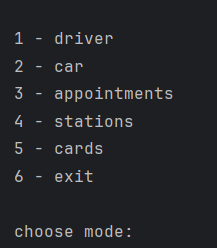
\includegraphics[width=.3\textwidth]{./db_edit_1.png}
    \caption{\en{main page}}
\end{figure}

\begin{figure}[H]
    \centering
    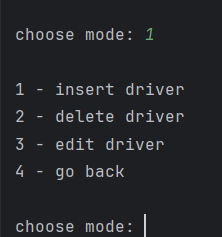
\includegraphics[width=.3\textwidth]{./db_edit_2.png}
    \caption{\en{main page}}
\end{figure}

\begin{figure}[H]
    \centering
    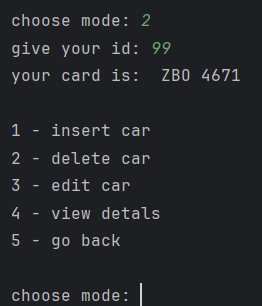
\includegraphics[width=.4\textwidth]{./db_edit_3.png}
    \caption{\en{main page}}
\end{figure}

\begin{figure}[H]
    \centering
    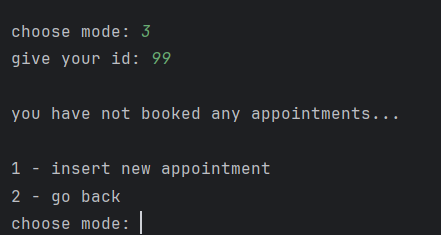
\includegraphics[width=.4\textwidth]{./db_edit_5.png}
    \caption{\en{main page}}
\end{figure}

\begin{figure}[H]
    \centering
    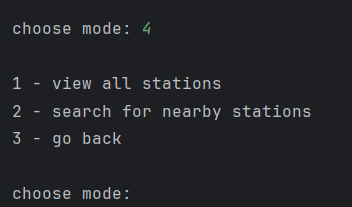
\includegraphics[width=.4\textwidth]{./db_edit_4.png}
    \caption{\en{main page}}
\end{figure}

\begin{figure}[H]
    \centering
    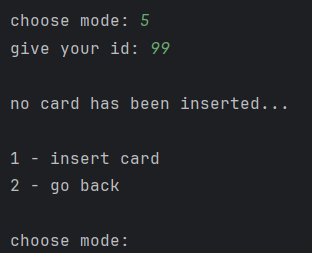
\includegraphics[width=.4\textwidth]{./db_edit_6.png}
    \caption{\en{main page}}
\end{figure}


\end{document}
\endinput
%%
%% End of file `sample-manuscript.tex'.

